\documentclass[12pt, a4paper]{article}

\usepackage[utf8]{inputenc}

% Limit the page margin to only 1 inch.
\usepackage[margin=1in]{geometry}

%Imports biblatex package
\usepackage[
backend=biber,
style=alphabetic
]{biblatex}
\addbibresource{../math-342w.bib}

% Enables the `align' environment.
\usepackage{amsmath}

% Provides useful environments, such as:
% - \begin{proof} ...\end{proof}
\usepackage{amsthm}
\newtheorem{proposition}{Proposition}
\theoremstyle{definition}
\newtheorem*{definition}{Definition}
\newtheorem{theorem}{Theorem}
\newtheorem{corollary}{Corollary}

% Enables using \mathbb{}, for example \mathbb{N} for the set of natural numbers.
\usepackage{amssymb}

% Allows using letters in enumerate list environment. Use, for example:
%\begin{enumerate}[label=(\alph*)]
% ...
%\end{enumerate}
\usepackage[inline]{enumitem}

% Enable importing external graphic files and provides useful commands, like \graphicspath{}
\usepackage{graphicx}
% Images are located in a directory called "images" in the current directory.
\graphicspath{{./images/}}

% Make links look better by default.
% See: https://tex.stackexchange.com/questions/823/remove-ugly-borders-around-clickable-cross-references-and-hyperlinks
\usepackage[hidelinks]{hyperref}
\usepackage{xcolor}
\hypersetup{
	colorlinks,
	linkcolor={red!50!black},
	citecolor={blue!50!black},
	urlcolor={blue!80!black}
}

% Code Listings. Source:
% https://stackoverflow.com/questions/3175105/inserting-code-in-this-latex-document-with-indentation
\usepackage{listings}
\usepackage{color}
\usepackage[most]{tcolorbox}

\definecolor{dkgreen}{rgb}{0,0.6,0}
\definecolor{gray}{rgb}{0.5,0.5,0.5}
\definecolor{mauve}{rgb}{0.58,0,0.82}

\lstset{frame=tb,
	language=Java,
	aboveskip=3mm,
	belowskip=3mm,
	showstringspaces=false,
	columns=flexible,
	basicstyle={\small\ttfamily},
	numbers=none,
	numberstyle=\tiny\color{gray},
	keywordstyle=\color{blue},
	commentstyle=\color{dkgreen},
	stringstyle=\color{mauve},
	breaklines=true,
	breakatwhitespace=true,
	tabsize=3
}

\newcommand{\prob}{\text{P}}
%\newcommand{\complement}{\mathsf{c}}
\title{Lecture 8: MATH 342W: Introduction to Data Science and Machine Learning}
\author{Sergio E. Garcia Tapia\thanks{Based on lectures of Dr. Adam Kapelner at Queens College.
See also the \href{https://github.com/kapelner/QC_MATH_342W_Spring_2025}{course GitHub page}.}}
\date{February 25, 2025 (last updated \today)}

\begin{document}
	\maketitle
	\subsection*{Recap}
	Last time, we began discussing multivariate linear ``regression", with
	$p>1$ features, $\mathcal{X}=\mathbb{R}^p$, and $\mathcal{Y}=\mathbb{R}$.
	Given a data set $\mathbb{D}=\{(\mathbf{x}_i, y_i)\}_{i=1}^{n}\subseteq \mathcal{X}\times \mathcal{Y}$,
	we were looking to predict using candidate functions that define a hyperplane. Recall this
	means we have an equation of the form
	\begin{align*}
		0&=w_0+w_1x_1+w_2x_2+\cdots+w_px_p\\
		 &= \begin{bmatrix}
			1 & x_1 & \cdots & x_p
		\end{bmatrix}^\top
		\begin{bmatrix}
			w_0 \\
			w_1\\
			\vdots\\
			w_p
		\end{bmatrix}\\
		&= \mathbf{x}^\top \mathbf{w}
	\end{align*}
	Because of this, we overloaded our notation for the observations $\mathbf{x}_i$, so that
	instead of denoting a $p$-dimensional vector, it denotes a $(p+1)$-dimensional vector
	whose first entry is $1$. Hence, for $\mathbf{x}\in \{1\}\times \mathbb{R}^{p}\subset \mathbb{R}^{p+1}$,
	the set of candidate functions is given by
	\begin{align*}
		\mathcal{H} = \{\mathbf{x}^\top \mathbf{w}=0: \mathbf{w}\in\mathbb{R}^{p+1}\}
	\end{align*}
	We defined $X$ to be a matrix of size $n\times (p+1)$, where the $i$th row consists
	of a $1$ entry followed by the entries of $\mathbf{x}_i$ (the $p$ features of the
	$i$th observation).
	\begin{align*}
		X := \begin{bmatrix}
			1 & x_{1,1} & x_{1, 2} & \cdots & x_{1, p}\\
			\vdots & \vdots & \vdots & \cdots & \vdots\\
			1 & x_{n, 1} & x_{n, 2} & \cdots& x_{n, p}
		\end{bmatrix}
	\end{align*}
	In other words, we make a matrix whose first column is $\vec{\mathbf{1}}_n$, and where
	every other observation in the feature space becomes a row. Note the $j$th column
	consists of the values of the $j$th feature across all $n$ observations.
	
	If $g\in\mathcal{H}$, then there is a fixed $\mathbf{w}\in\mathbb{R}^{p+1}$ such
	that $\hat{y}_i=g(\mathbf{x}_i)=\mathbf{w}^T\mathbf{x}_i$. Equivalently, since
	$\hat{y}_i$ is a scalar, and we think of $\hat{y}_i$ as the $1\times 1$ matrix $[\hat{y_i}]$, then
	$\hat{y}_i=\hat{y}_i^\top$ (equals its transpose), so
	\begin{align*}
		\hat{y}_i=\hat{y}_i^\top = (\mathbf{w}^\top \mathbf{x}_i)^\top = \mathbf{x}_i^\top \mathbf{w},\quad
		\forall i
	\end{align*}
	Recall that we can think of the $i$th row of the matrix product $A\mathbf{u}$ as the
	dot product of the $i$th row of $A$ and $\mathbf{u}$. If we let $\hat{\mathbf{y}}$ be
	the prediction vector obtained by applying $g$ to the $\mathbf{x}_i$ in $\mathbb{D}$, then
	\begin{align*}
		\hat{\mathbf{y}} := \begin{bmatrix}
			\hat{y}_1\\
			\vdots\\
			\hat{y}_n
		\end{bmatrix}
		=
		\begin{bmatrix}
			\mathbf{x}_1^\top \mathbf{w}\\
			\vdots\\
			\mathbf{x}_n^\top \mathbf{w}
		\end{bmatrix}
		=X\mathbf{w}
	\end{align*}
	Define the response vector
	\begin{align*}
	\mathbf{y}:=\begin{bmatrix}
		y_1\\
		y_2\\
		\vdots\\
		y_n
	\end{bmatrix}
	\end{align*}
	Then the error (residual) is given by $\mathbf{e}:=\mathbf{y}-\hat{\mathbf{y}}$,
	and in order to obtain the best $g$ (the least squares approximation), we need
	to minimize the $SSE$, which is given by
	\begin{align}
		SSE &= \sum_{i=1}^{n}e_i^2\nonumber\\
		&=\mathbf{e}^\top \mathbf{e}\nonumber\\
		&=\mathbf{y}^\top\mathbf{y} - 2\mathbf{y}^TX\mathbf{w}+
		+\mathbf{w}^\top X^\top X \mathbf{w}.
		\label{eqn:sse-objective}
	\end{align}
	We will present some results from calculus and linear algebra that will help us tackle
	this problem.
	\subsection*{Interlude of Linear Algebra and Calculus}
	\begin{tcolorbox}
		\begin{proposition}
			Let $\mathbf{x}\in\mathbb{R}^n$, and let $a\in\mathbb{R}$ be a constant with
			respect to all entries of $\mathbf{x}$. Then
			\begin{align}
				\frac{\partial}{\partial\mathbf{x}}[a] := \begin{bmatrix}
					\frac{\partial}{\partial x_1}[a]\\
					\frac{\partial}{\partial x_2}[a]\\
					\vdots\\
					\frac{\partial}{\partial x_n}[a]
				\end{bmatrix}
				=\begin{bmatrix}
					0\\
					0\\
					\vdots\\
					0
				\end{bmatrix}
				=\mathbf{0}_{n}
				\label{eqn:deriv-constant}
			\end{align}
		\end{proposition}
	\end{tcolorbox}
	\begin{tcolorbox}
		\begin{proposition}
			Let $\mathbf{a}\in\mathbb{R}^n$, where all entries are constant with respect to
			all entries of $\mathbf{x}$. Then
			\begin{align}
				\frac{\partial}{\partial\mathbf{x}}[\mathbf{a}\cdot \mathbf{x}]=
				\frac{\partial}{\partial \mathbf{x}}[\mathbf{a}^\top \mathbf{x}]=\mathbf{a}
				\label{eqn:deriv-const-dot}
			\end{align}
		\end{proposition}
	\end{tcolorbox}
	\begin{tcolorbox}
		\begin{proposition}
			Let $\mathbf{x}\in\mathbb{R}^n$, $a,b\in\mathbb{R}$, and $f,g:\mathbb{R}^n\to\mathbb{R}$
			be differentiable functions. Then
			\begin{align}
				\frac{\partial}{\partial \mathbf{x}}[af(\mathbf{x}) + b g(\mathbf{x})]
				= a \cdot \frac{\partial}{\partial \mathbf{x}} [f(\mathbf{x})]
				+ b \cdot \frac{\partial}{\partial \mathbf{x}} [g(\mathbf{x})]
				\label{eqn:deriv-of-sum}
			\end{align}
			In other words, the derivative is linear for differentiable functions of several variables.
		\end{proposition}
	\end{tcolorbox}
	
	\begin{tcolorbox}
		\begin{proposition}
			Let $A$ be an $n\times n$ matrix ($A\in\mathbb{R}^{n\times n}$) that is symmetric
			(recall this means $a_{i,j}=a_{j,i}$ for all $i, j$), and whose entries are all
			constant with respect to $\mathbf{x}\in\mathbb{R}^n$. Then
			\begin{align}
				\frac{\partial }{\partial\mathbf{x}}[\mathbf{x}^\top A\mathbf{x}] = 2\cdot A\mathbf{x}
				\label{eqn:deriv-quad-form}
			\end{align}
			\textbf{Remark}: The expression $\mathbf{x}^\top A\mathbf{x}$ is a scalar, and the
			form of this product is known as a \textbf{quadratic form}. Perhaps the name is
			from the fact that it resembles $\frac{d}{dx}(ax^2)=2ax$, where $a,x\in\mathbb{R}$.
		\end{proposition}
	\end{tcolorbox}
	
	\subsection*{Minimizing the $SSE$ in Multivariate Least Squares}
	We can now return to our main goal, which is a minimization problem
	\begin{align*}
		\mathcal{A}:\mathbf{b} = \underset{\mathbf{w}\in\mathbb{R}^{p+1}}{\text{argmin}}\{SSE(\mathbf{w})\}
	\end{align*}
	Consider Equation~\ref{eqn:sse-objective}, and note the following observations:
	\begin{itemize}
		\item $\mathbf{y}^T\mathbf{y}$ is constant with respect to $\mathbf{w}$.
		\item Using the property that $(AB)^\top = B^\top A^\top$, we can write
		$\mathbf{y}^\top X = (X^\top \mathbf{y})^\top$.
		\item The matrix $X^\top X$ is symmetric: $(X^\top X)^\top = X^\top (X^\top)^\top=X^\top X$.
	\end{itemize}
	We proceed to taking the derivative with respect to
	$\mathbf{w}\in\mathbb{R}^{p+1}$ and using the equations from our interlude along with our
	observations above:
	\begin{align*}
		\frac{\partial}{\partial \mathbf{w}}[SSE]
		&= \frac{\partial}{\partial \mathbf{w}}[
		\mathbf{y}^\top \mathbf{y} - 2\mathbf{y}^\top X \mathbf{w} + \mathbf{w}^\top X^\top X \mathbf{w}
		]\\
		&\underbrace{=}_{\text{Eqn~\ref{eqn:deriv-of-sum}}}\underbrace{\frac{\partial}{\partial \mathbf{w}}[\mathbf{y}^\top \mathbf{w}]}_{\text{Eqn~\ref{eqn:deriv-constant}}}
		-2\underbrace{\frac{\partial}{\partial \mathbf{w}}[(X^\top \mathbf{y})^\top\mathbf{w}]}_{\text{Eqn~\ref{eqn:deriv-const-dot}}}
		+\underbrace{\frac{\partial}{\partial \mathbf{w}}[\mathbf{w}^\top X^\top X\mathbf{w}]}_{\text{Eqn~\ref{eqn:deriv-quad-form}}}\\
		&= \mathbf{0}_{p+1} - 2\cdot X^\top \mathbf{y} + 2\cdot X^\top X\mathbf{w}
	\end{align*}
	If we set it to $\mathbf{0}_{p+1}$, then the solution is the vector $\mathbf{w}=\mathbf{b}$
	that minimizes the $SSE$.
	\begin{align*}
		\mathbf{0}_{p+1} &= - 2\cdot X^\top \mathbf{y} + 2\cdot X^\top X\mathbf{b}\\
		X^\top X\mathbf{b} &= X^\top \mathbf{y}
	\end{align*}
	Suppose for now that the matrix $X^\top X$ of size $(p+1)\times(p+1)$ is invertible.
	Then the solution is given by
	\begin{align}
		\mathbf{b} = (X^\top X)^{-1}X^\top\mathbf{y}\label{eqn:multivar-ols-coeffs}
	\end{align}
	For $X^\top X$ to be invertible, it must have full-rank. Since $X^\top X$ has $p+1$
	columns, this means we need $\text{rank}(X^\top X)= p + 1$, where the rank denotes
	the dimension of the range of $X^\top X$. We will show an equivalent condition
	for $X^\top X$ to have full rank, but first here's a theorem from linear algebra:
	\begin{tcolorbox}[breakable]
		\begin{theorem}[Fundamental Theorem of Liner Maps, or Rank-Nullity Theorem]
			\label{thm:rank-nullity}
			Let $V$ and $W$ be vector spaces, where $V$ is finite-dimensional, and let
			$T:V\to W$ be a linear transformation. Then
			\begin{align*}
				\dim \text{range}(T) + \dim \text{null}(T) = \dim V
			\end{align*}
		\end{theorem}
	\end{tcolorbox}
	See \cite{axler}\footnote{See Open Access edition at https://linear.axler.net/LADR4e.pdf} for a proof of Theorem~\ref{thm:rank-nullity}.
	Now we can show:
	\begin{tcolorbox}[breakable]
		\begin{theorem}
			\label{thm:rank-XTX}
			Given any matrix $\mathbf{X}$ of dimension $n\times (p+1)$, we have
			\begin{align*}
				\text{rank}(X^\top X)= \text{rank}(X)
			\end{align*}
		\end{theorem}
		\begin{proof}
			Our strategy is to show that $X^T$ and $X$ have the same null space, and then use
			Theorem~\ref{thm:rank-nullity}. Let $\mathbf{v}\in \text{null}(X^\top X)$,
			so that $(X^\top X)\mathbf{v}=\mathbf{0}_{p+1}$. Multiply by $\mathbf{v}^\top$
			on the left to get:
			\begin{align*}
				\mathbf{v}^\top X^\top X\mathbf{v} &= \mathbf{v}^\top \mathbf{0}_{p+1}\\
				(X\mathbf{v})^\top (X\mathbf{v}) &= 0\\
			\end{align*}
			Notice this says that the dot product of $X\mathbf{v}$ with itself is $0$,
			which implies $X\mathbf{v}=\mathbf{0}_n$. Hence, $\mathbf{v}\in \text{null}(X)$,
			proving that $\text{null}(X^\top X)\subseteq \text{null}(X)$.
			
			For the other direction, suppose now that $\mathbf{v}\in \text{null} X$, so
			that $X\mathbf{v}=\mathbf{0}_n$. Then multiplying on the left by $X^\top$ gives
			$X^\top X\mathbf{v}=X^\top \mathbf{0}_{n}=\mathbf{0}_{p+1}$, so
			$\mathbf{v}\in \text{null}(X^\top X)$, and hence $\text{null}(X)\subseteq \text{null}(X^\top X)$.
			
			We conclude that $\text{null}(X^\top X)=\text{null}(X)$, and hence their dimensions
			are the same. Now we will apply Theorem~\ref{thm:rank-nullity} to both $X$ and $X^\top X$.
			Note that the domain space for both $X$ and $X^\top X$ is $\mathbb{R}^{p+1}$, so
			\begin{align*}
				\dim \text{range}(X) + \dim\text{null}(X) &= \dim \mathbb{R}^{p+1}\\
				\dim \text{range}(X^\top X) + \dim\text{null}(X^\top X) &= \dim \mathbb{R}^{p+1}\\
			\end{align*}
			If we subtract both equations, we arrive at $\dim \text{range}(X)=\dim\text{range}(X^\top X)$.
			Since the dimension of the range is precisely the rank, we are done.
		\end{proof}
	\end{tcolorbox}
	From Theorem~\ref{thm:rank-XTX}, we see that
	\begin{align*}
		X^\top X\text{is invertible } &\iff \text{rank}(X^TX)=p+1\\
		&\iff \text{rank}(X)=p+1\\
		&\iff \text{all columns of $X$ are linearly independent.}
	\end{align*}
	What does this last fact mean? It means that \textit{none of the $p+1$ features are ``redundant"}.
	For example, if we measured height in feet and in meters, and included a feature for each
	measurement, then our columns would be linearly dependent, and $X$ would not be full rank
	(and hence $X^\top X$ is not invertible). In practice, we do not worry much about this because
	we can feed our matrix into a computer that can determine the rank and compute the inverse for us.
	
	\subsection*{Performance Metrics for Multivariate Ordinary Least Squares}
	Let's revisit the error measures for OLS:
	\begin{align*}
		SSE &:= \mathbf{e}^\top \mathbf{e}\\
		MSE &:= \frac{1}{n-(p+1)}SSE\\
		RMSE &:= \sqrt{MSE}\\
		R^2 &:= 1 - \frac{SSE}{SST}
	\end{align*}
	The only one that has changed appearance is the $MSE$. Notice that if $p=1$, then
	we recover the simple OLS formula for $MSE$. The quantity $p+1$ is known as
	the \textbf{number of degrees of freedom (df)}. That is, $df = \text{rank}(X)=p+1$.
	An interesting observation is that if $p$ is high, then the $MSE$ increases, so the
	average squared error is penalized for having more features. We will explore this
	further later on.
	\subsection*{Least Squares Estimates}
	We see that the least square estimate is given by Equation~\ref{eqn:multivar-ols-coeffs}.
	Therefore, if $\mathbf{x}_*\in\mathbb{R}^{p+1}$ (recall we pre-pend a $1$) is an incoming
	observation for which we would like to predict a response, we can do so via a dot product:
	\begin{align*}
		\hat{y}_* = g(\mathbf{x}_*) = \mathbf{x}_*^\top \mathbf{b}
	\end{align*}
	More generally, if we have $n_*$ observations, we can create an $n_*\times (p+1)$ matrix
	$X_*$ similar to $X$ (first column is $\vec{\mathbf{1}}_*$) where the $i$th row contains the $i$th observation,
	and we can predict for all values at once using matrix multiplication:
	\begin{align*}
		\hat{\mathbf{y}}_*=\begin{bmatrix}
			\hat{y}_{1, *}\\
			\vdots\\
			\hat{y}_{n_*, *}
		\end{bmatrix}
		=\begin{bmatrix}
			\mathbf{x}_{*, 1}^\top \mathbf{b}\\
			\vdots\\
			\mathbf{x}_{*, n}^\top \mathbf{b}
		\end{bmatrix}
		=X_* \mathbf{b}
	\end{align*}
	What if we don't have any features? That is, we have $p=0$ and $n$ observations,
	and the $n\times (p+1)$ matrix $X$ only has the first column of $1$'s. In this case,
	$X =\vec{\mathbf{1}}_n$. Since $\mathbf{b}$ is length $p+1$ and $p=0$,
	it has a single entry, and hence
	\begin{align*}
		\mathbf{b} &= b_0\\
		& = (X^\top X)^{-1} X^\top \mathbf{y}\\
		&=(\vec{\mathbf{1}}_n^\top \vec{\mathbf{1}}_n)^{-1} \vec{\mathbf{1}}_n^\top\mathbf{y}\\
		&=(n)^{-1}\sum_{i=1}^{n}y_i\\
		&=\bar{y}
	\end{align*}
	Hence, the \textbf{null model} is given by
	\begin{align*}
		g_0(\mathbf{x}_*)=\bar{y} \quad \text{ for all }\mathbf{x}_*\in \{1\} \times \mathbb{R}^{p},
	\end{align*}
	and it is a least squares estimate because we obtained it by using the least squares formula.
	\subsection*{The Hat Matrix}
	In linear algebra we learn that a useful (and correct) way to think about matrix
	multiplication $A\mathbf{u}$ is as a linear combination of the columns of $A$ using the
	entries in $\mathbf{u}$ as coefficients. For example if $A$ is an $n\times p$ matrix,
	and ${A}_{\cdot, 1},\ldots,{A}_{\cdot, p}$ are the $p$ columns
	of $A$, then
	\begin{align*}
		A\mathbf{u}=u_1 A_{\cdot, 1} + \cdots + u_p A_{\cdot, p}
	\end{align*}
	In particular, $A\mathbf{u}\in co\ell(A)=\text{span}(A_{\cdot, 1},\ldots,A_{\cdot, p})$.
	Similarly, in the equation for the predictions $\hat{\mathbf{y}}=X\mathbf{b}$,
	we see that $\hat{\mathbf{y}}$ is a linear combinations of the $p+1$ columns
	of $X$. We are assuming that $X$ is a $n\times (p+1)$ full rank matrix with
	$p + 1 < n$, so full rank means that $\dim co\ell (X) = p+1$. Therefore,
	it follows that $\hat{\mathbf{y}}$ belongs to a $(p+1)$-dimensional subspace
	of $\mathbb{R}^n$.
	
	Let's expand the expression for $\hat{\mathbf{y}}$ using Equation~\ref{eqn:multivar-ols-coeffs}:
	\begin{align}
		\hat{\mathbf{y}} &= X \mathbf{b}\nonumber\\
		&=X(X^\top X)^{-1}X^\top  \mathbf{y}\nonumber\\
		&=\underbrace{(X(X^\top X)^{-1} X^\top)}_{H}\mathbf{y}\nonumber\\
		&=H\mathbf{y}\label{eqn:hat-matrix}
	\end{align}
	The $n\times n$ matrix $H$ is called the \textbf{Hat matrix}. It turns out
	that $\text{rank}(H) = p +1$, which we can argue as follows.
	
	Suppose that
	$\mathbf{v}\in \text{null}(H)$, so that $H\mathbf{v}=0$. By associativity
	of matrix multiplication, this means $X((X^\top X)X^{-1}\mathbf{v})=0$.
	Since $X$ has full rank $(p+1)$, this means it is injective, and hence
	$(X^\top X)X^{-1}\mathbf{v}=0$. Similarly, associativity says this is equivalent
	to $(X^\top X)(X^\top\mathbf{v})=0$. By Theorem~$\ref{thm:rank-XTX}$, $X^\top X$
	also has rank $p+1$, so it is full rank and hence injective. Thus, we must have
	$X^\top\mathbf{v}=0$. In other words, $\text{null}(H)\subseteq \text{null}(X^\top)$.
	It's easy to see that $\text{null}(X^\top)\subseteq \text{null}(H)$ by definition of
	$H$, so their null spaces are of the same size and hence $\dim \text{null}(H) = \dim\text{null}(X^\top)$.
	Since $\text{rank}(X^\top)=\text{rank}(X)=p+1$, we can invoke Theorem~\ref{thm:rank-nullity}
	to write
	\begin{align*}
		\text{rank}(X^\top) + \dim\text{null}(X^\top) &= n\\
		\text{rank}(H) + \dim\text{null}(H) &= n
	\end{align*}
	Subtracting both equations, we arrive at $\text{rank}(H) = p+1$. Again, this hinges
	on $X$ being $n\times (p+1)$, of rank $p+1$, and $p+1 < n$. In particular, $H$
	is not invertible. Later on, we consider the case where $p+1 > n$.
	\subsection*{Orthogonal Projections}
	Let $\mathcal{V}$ be a $k$-dimensional subspace of $\mathbb{R}^n$, where $k\leq n$.
	Then
	\begin{align*}
	\mathcal{V}=\text{span}(\mathbf{v}_1,\mathbf{v}_2\ldots,\mathbf{v}_k)
	\end{align*}
	for $\mathbf{v}_1,\ldots,\mathbf{v}_k\in\mathbb{R}^n$, and the vectors form a linearly
	independent list. Let $\mathbf{a}\in\mathbb{R}^n$, and consider the projection
	$\mathbf{a}$ onto $V$, denoted $\text{proj}_\mathcal{V}(\mathbf{a})$, which is a vector
	in $\mathcal{V}$ such that the difference $\mathbf{a} - \text{proj}_V(\mathbf{a})$ is
	perpendicular to $\mathcal{V}$. Think of $\text{proj}_{\mathcal{V}}(\mathbf{a})$ as the
	shadow of $\mathbf{a}$ along $\mathcal{V}$. See Figure~\ref{fig:orthogonal-projection}.
	\begin{figure}
		\centering
		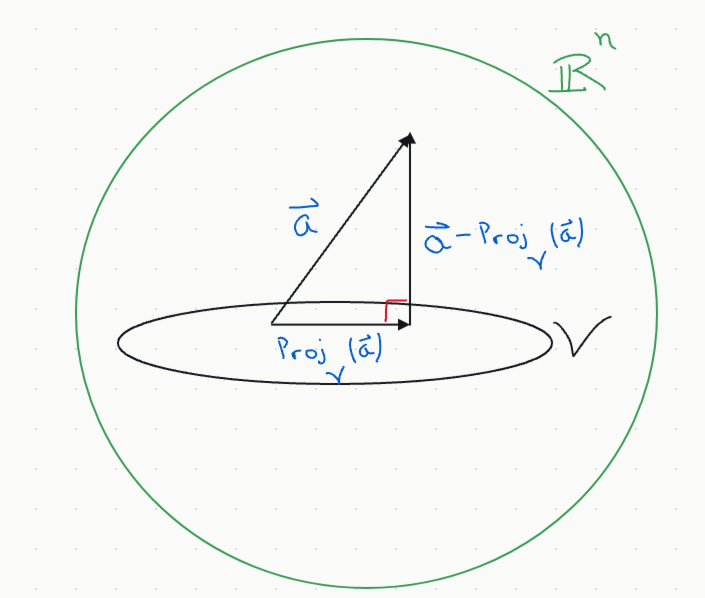
\includegraphics[width=0.6\textwidth]{orthogonal-projection}
		\caption{Orthogonal projection of a vector $\mathbf{a}$ in $\mathbb{R}^n$ onto
		a $k$-dimensional subspace $V$ of $\mathbb{R}$.}
		\label{fig:orthogonal-projection}
	\end{figure}
	This is called an \textbf{orthogonal projection}.
	
	Since $\text{proj}_\mathcal{V}(\mathbf{a})\in \mathcal{V}$, there are coefficients
	$w_1,\ldots,w_k$ such that
	\begin{align*}
		\text{proj}_\mathcal{V}(\mathbf{a}) = w_1\mathbf{v}_1+w_2\mathbf{v}_2+\cdots+w_k\mathbf{v}_k
	\end{align*}
	Let $V$ denote a matrix whose columns are the vectors $\mathbf{v}_1,\ldots,\mathbf{v}_k$ that
	we said span $\mathcal{V}$ (in fact they form a basis), and $\mathbf{w}$ be a $k$-length
	vector from the $w_i$ coefficients:
	\begin{align*}
		V = \begin{bmatrix}
			\vdots & \cdots& \vdots\\
			\mathbf{v}_1 & \cdots& \mathbf{v}_k\\
			\vdots& \cdots & \vdots
		\end{bmatrix},\quad
		\mathbf{w} = \begin{bmatrix}
			w_1\\
			w_2\\
			\vdots\\
			w_k
		\end{bmatrix}
	\end{align*}
	Then we can express the projection as a matrix multiplication:
	\begin{align}
		\text{proj}_{\mathcal{V}}(\mathbf{a})=V\mathbf{w}\label{eqn:proj-system}
	\end{align}
	Moreover, since $\mathbf{a}-\text{proj}_{\mathcal{V}}(\mathbf{a})\in \mathcal{V}^\perp$
	(the orthogonal complement), it follows that for all $\mathbf{v}_j$ we have
	\begin{align*}
		0 &=\mathbf{v}_j^\top (\mathbf{a}-\text{proj}_{\mathcal{V}}(\mathbf{a}))\\
		&=\mathbf{v}_j^\top(\mathbf{a}-V\mathbf{w})
	\end{align*}
	Since the equation above holds for all $j$, we can write it as a matrix multiplication:
	\begin{align*}
		V^\top(\mathbf{a} - V\mathbf{w}) &= \mathbf{0}_k
	\end{align*}
	To see why, note that since we think of $\mathbf{v}_j$ as a column vector, the $j$th row of $V^\top$ 
	is $\mathbf{v}_j^\top$, and product of $V^\top$ and $(\mathbf{a}-V \mathbf{w})$ is precisely
	the product of each row of $V^\top$ with $\mathbf{a}-V\mathbf{w}$. Now we can expand and
	solve for $\mathbf{w}$:
	\begin{align}
		V^\top \mathbf{a} - V^\top V\mathbf{w} &= \mathbf{0}_{k}\nonumber\\
		V^\top V \mathbf{w} &= V^\top \mathbf{a}\nonumber\\
		\mathbf{w} &= (V^\top V)^{-1} V^\top \mathbf{a}\label{eqn:proj-coeffs}
	\end{align}
	The last step requires that $V^\top V$ be invertible, and we argue that it is.
	To see why, recall that by Theorem~\ref{thm:rank-XTX}, $\text{rank}[V^\top V] = \text{rank}[V]$,
	and since $V$ is made up of $k$ linearly independent vectors, $\mathbf{v}_1,\ldots,\mathbf{v}_k$,
	its rank is $k$. Hence, $\text{rank}[V^\top V]=k$, and it has size $k\times k$, so it is
	invertible.
	
	Now that we have determined the coefficients $\mathbf{w}$ used to write
	$\text{proj}_{\mathcal{V}}(\mathbf{a})$ in terms of the basis of $\mathcal{V}$,
	we can combine Equations~\ref{eqn:proj-system} and ~\ref{eqn:proj-coeffs}:
	\begin{align}
		\text{proj}_{\mathcal{V}}(\mathbf{a})=V(V^\top V)^{-1}V^\top \mathbf{a}\label{eqn:orthon-proj-matrix}
	\end{align}
	The matrix $V(V^\top V)^{-1}V^\top$ is called an \textbf{orthogonal projection matrix}.
	This resembles the Hat matrix in Equation~\ref{eqn:hat-matrix}. Indeed, this implies
	that the Hat matrix $H$ is an orthogonal projection matrix, and given the expression
	$\hat{\mathbf{y}}=H\mathbf{y}$, it says that $\hat{\mathbf{y}}$ is the orthogonal projection
	of $\mathbf{y}$ onto the column space of $H$, which in turn is the column space of $X$:
	\begin{align*}
		\hat{\mathbf{y}} = \underset{co\ell[X]}{\text{proj}}(\mathbf{y})
	\end{align*}
	See Figure~\ref{fig:prediction-space}.
	\begin{figure}
		\centering
		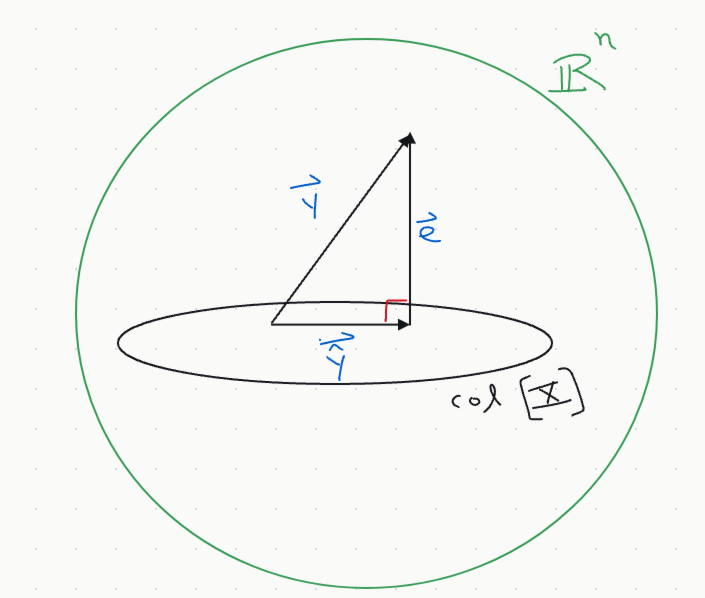
\includegraphics[width=0.4\textwidth]{prediction-orthogonal-projection}
		\caption{The prediction $\hat{\mathbf{y}}$ viewed as an orthogonal
			projection of the response vector $\mathbf{y}$ onto the column space of $X$.}
		\label{fig:prediction-space}
	\end{figure}
	Recall the residual is defined as $\mathbf{e}:=\mathbf{y}-\hat{\mathbf{y}}$.
	Using Equation~\ref{eqn:hat-matrix}, we can write
	\begin{align}
		\mathbf{e}:=\mathbf{y}-\hat{\mathbf{y}}=\mathbf{y}-H\mathbf{y} = (I-H)\mathbf{y}
	\end{align}
	Though we will not show it this time, the matrix $I-H$ is also an
	orthogonal projection matrix. This time, we are projecting onto the ``residual space".
	See Figure~\ref{fig:residual-space}.
	\begin{figure}
		\centering
		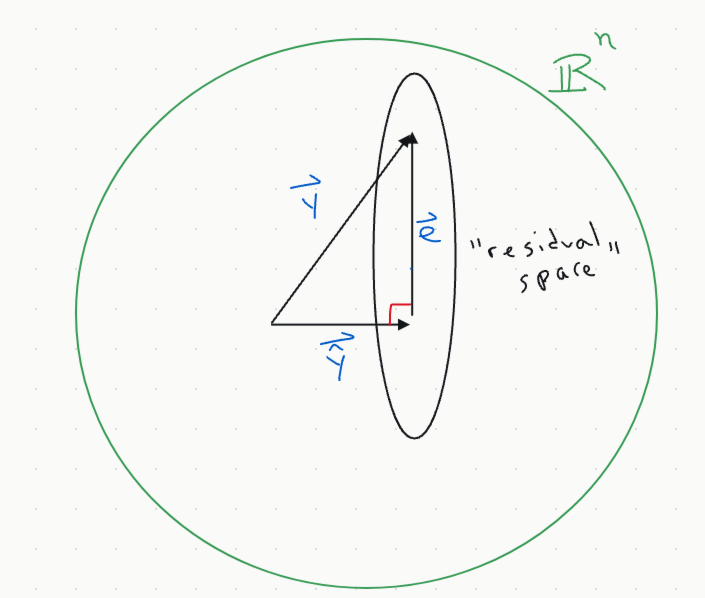
\includegraphics[width=0.4\textwidth]{residual-space}
		\caption{The residual $\mathbf{e}$ viewed as an orthogonal
			projection of the response vector $\mathbf{y}$ onto the ``residual space".}
		\label{fig:residual-space}
	\end{figure}
	In fact, a theorem in linear algebra says that the space $co\ell [X]\cap  (co\ell[X])^\perp=\{0\}$,
	and their sum is the entire space, so we have the direct sum:
	\begin{align*}
		co\ell [X]\oplus (co\ell [X])^\perp = \mathbb{R}^n
	\end{align*}
	See Chapter 6 in \cite{axler}. In particular, we imagine that if we put the bases
	for both of these space together, we get a fuller matrix as in Figure~\ref{fig:mat-ortho-decomp}.
	\begin{figure}
		\centering
		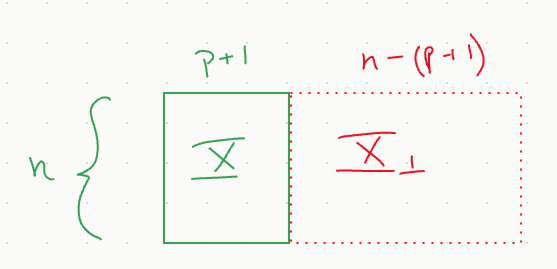
\includegraphics[width=0.4\textwidth]{matrix-orthogonal-decomposition}
		\caption{Matrix from putting the bases of $co\ell [X]$ and $(co\ell[X])^\perp$ together.}
		\label{fig:mat-ortho-decomp}
	\end{figure}
	\pagebreak
	\printbibliography
\end{document}